\documentclass{article}

\usepackage{graphicx}
\usepackage{tikz}
\usepackage{tikzsymbols}
\usetikzlibrary{calc,patterns,shapes.geometric}
\pagestyle{empty}
\usepackage[margin=0pt]{geometry}
\geometry{papersize={14in,12in}}

\def\centerarc[#1](#2)(#3:#4:#5){\draw[#1] ($(#2)+({#5*cos(#3)},{#5*sin(#3)})$) arc (#3:#4:#5);}

\begin{document}
	\begin{figure}
		\centering
		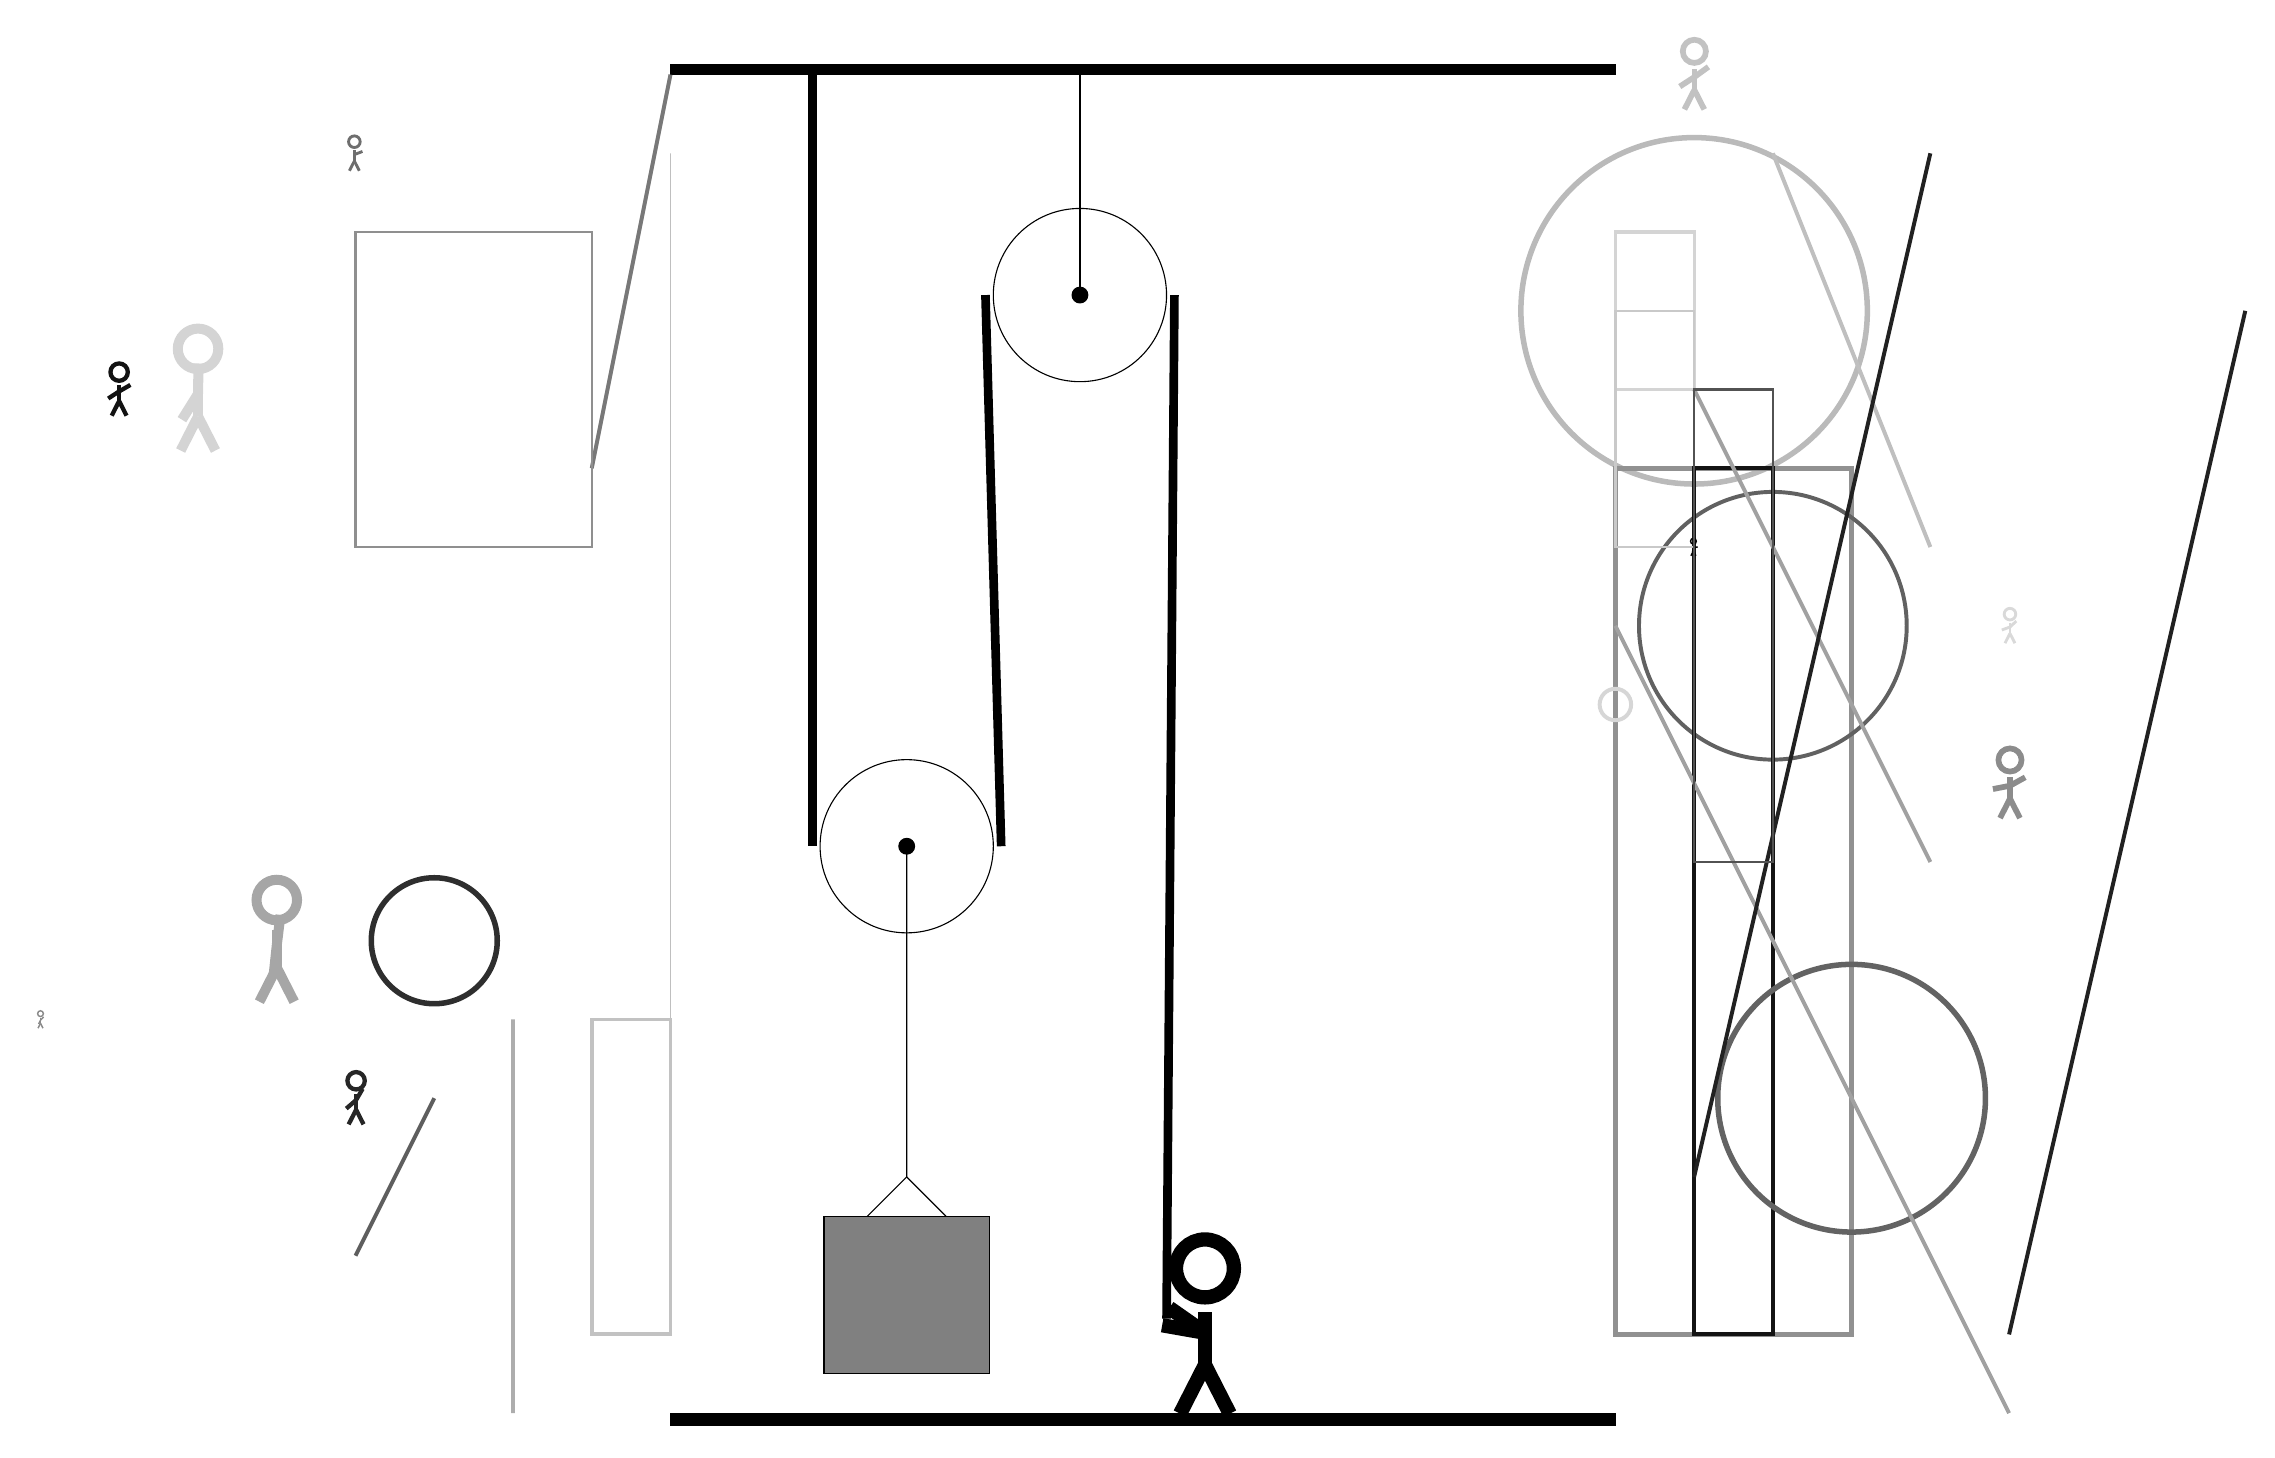
\begin{tikzpicture}
			%%%%% START %%%%%
			
			\draw[fill=black] (-2, 14) rectangle (10, 14.125);
			
			\draw (3.2, 11.2) circle (1.1);
			\draw[fill=black] (3.2, 11.2) circle (0.1);
			\draw[thick] (3.2, 11.2) -- (3.2, 14);
			
			\draw (1, 4.2) circle (1.1);
			\draw[fill=black] (1, 4.2) circle (0.1);
			
			\draw [line width=0.7mm, color=black!27](11, 11) circle (2.2);
			
			\draw[line width=0.7mm, color=black!43] (10, 9) rectangle (13, -2);
			\draw [line width=0.7mm, color=black!82](-5, 3) circle (0.8);
			\node[line width=0.7mm, color=black!46] at (-10, 2) {\Strichmaxerl[1][64][46]};
			\draw [line width=0.5mm, color=black!16](10, 6) circle (0.2);
			
			\node[line width=0.6mm, color=black!35] at (-7, 3) {\Strichmaxerl[7][84][83]};
			
			\draw[line width=0.4mm, color=black!17] (11, 12) rectangle (10, 10);
			
			\draw[line width=0.5mm, color=black!53](-2, 14) -- (-3, 9);
			\node[line width=0.3mm, color=black!57] at (-6, 13) {\Strichmaxerl[2][90][21]};
			
			\node[line width=0.6mm, color=black!45] at (15, 5) {\Strichmaxerl[4][11][29]};
			\draw[line width=0.5mm, color=black!87](15, -2) -- (18, 11);
			
			\node[line width=0.6mm, color=black!85] at (-6, 1) {\Strichmaxerl[3][41][60]};
			\draw[line width=0.2mm, color=black!25] (-2, 13) rectangle (-2, -2);
			
			\draw [line width=0.5mm, color=black!62](12, 7) circle (1.7);
			\draw[line width=0.5mm, color=black!92] (11, -2) rectangle (12, 9);
			\draw[line width=0.5mm, color=black!32] (-4, -3) rectangle (-4, 2);
			
			\draw[line width=0.5mm, color=black!25](14, 8) -- (12, 13);
			\draw[line width=0.5mm, color=black!24] (-2, 2) rectangle (-3, -2);
			\draw[line width=0.5mm, color=black!63](-6, -1) -- (-5, 1);
			\node[line width=0.4mm, color=black!15] at (15, 7) {\Strichmaxerl[2][20][43]};
			\draw [line width=0.7mm, color=black!61](13, 1) circle (1.7);
			\draw[line width=0.5mm, color=black!37](15, -3) -- (10, 7);
			\draw[line width=0.3mm, color=black!21] (10, 11) rectangle (11, 8);
			\draw[line width=0.5mm, color=black!37](11, 10) -- (14, 4);
			\node[line width=0.7mm, color=black!93] at (-9, 10) {\Strichmaxerl[3][33][30]};
			\draw[line width=0.3mm, color=black!44] (-3, 8) rectangle (-6, 12);
			\draw[line width=0.5mm, color=black!87](11, 0) -- (14, 13);
			\node[line width=0.4mm, color=black!99] at (11, 8) {\Strichmaxerl[1][79][10]};
			\draw[line width=0.3mm, color=black!68] (12, 4) rectangle (11, 10);
			\node[line width=0.7mm, color=black!17] at (-8, 10) {\Strichmaxerl[7][58][89]};
			\node[line width=0.3mm, color=black!24] at (11, 14) {\Strichmaxerl[4][33][36]};
			
			
			\draw (1, 4.2) -- (1, 0) -- (0.5, -0.5);
			\draw (1, 0) -- (1.5, -0.5);
			\draw[fill=black!50] (-0.05, -0.5) rectangle (2.05, -2.5);
			
			\draw[line width=1.1mm] (-0.2, 14) -- (-0.2, 4.2);
			\centerarc[line width=1.1mm](1, 4.2)(180:360:1.2000000000000002);
			\draw[line width=1.1mm](2.2, 4.2) -- (2.0, 11.2);
			\centerarc[line width=1.1mm](3.2, 11.2)(0:180:1.2000000000000002);
			\draw[line width=1.1mm](4.4, 11.2) -- (4.3, -1.8);
			
			\node at (4.7, -1.9) {\Strichmaxerl[10][-35][170]};
			
			\draw[fill=black] (-2, -3) rectangle (10, -3.15);
			
			%%%%% END %%%%%
		\end{tikzpicture}
	\end{figure}	
\end{document}